\documentclass[conference]{IEEEtran}
\usepackage[T1]{fontenc}
\usepackage{graphicx}
\usepackage{booktabs}
\usepackage{url}
\usepackage{cite}
\usepackage[hidelinks]{hyperref}
\urlstyle{same}
\raggedbottom
\pagestyle{plain}
\graphicspath{{figures/}}
\begin{document}
\title{Circuit Switchers: Direct-Mapped Cache Controller\\\large Modern Computer Architecture - Project 6}
\author{\IEEEauthorblockN{Guru Manohar Gupta, Harsith Priyan, Pranavi Mathur\\Yatin Singh, Dadi Dinesh}
\IEEEauthorblockA{Department of CS and AI\\Newton School of Technology\\Phase I -- 12 November 2026}}
\maketitle
\begin{abstract}
Processor performance can be limited by the time required to access main memory. A cache retains recently used blocks near the processor and can exploit temporal and spatial locality. Circuit Switchers proposes a direct-mapped, read-only cache controller in Verilog with 32-bit byte addresses, 1024 bytes of data capacity, 64 lines and 16-byte blocks. Direct mapping provides a simple indexed lookup and a deterministic replacement location. The Phase-I prototype implements the address decoder and the data, tag and valid-bit storage; a top-level skeleton establishes the remaining interfaces. Re-executed Icarus Verilog simulations passed six directed decoder cases and 22 storage checks. Stub-assisted elaboration verifies module-port compatibility only. Functional lookup, byte selection, controller sequencing, main-memory service and integrated-system verification remain pending. This report presents the implemented architecture, the proposed transaction flow, verified component evidence and the five-member work allocation without claiming completed cache operation or measured performance gains.
\end{abstract}
\begin{IEEEkeywords}direct-mapped cache, Verilog, memory hierarchy, RTL verification, Phase-I prototype\end{IEEEkeywords}
\section{Introduction}
Memory hierarchy design balances access latency, capacity and cost \cite{smith1982}, \cite{hennessy2017}. Caches exploit temporal reuse and nearby accesses. A hit serves a request from an existing line; a miss requires a lower memory level. Benefits depend on workload and implementation timing and must be measured.

Circuit Switchers is a five-member Modern Computer Architecture project. Its initial scope is one outstanding read, an 8-bit response, synchronous active-high reset and aligned 128-bit refill. Writes, coherence and physical DRAM integration are outside this milestone. This report audits baseline commit \path{370a8f7}, with component tests rerun on 12 November 2026. Documentation changes do not alter the RTL. The submission deadline is 16 November 2026.

\section{Literature Review}
\subsection{Memory hierarchy and locality}
Smith's survey examines cache placement, replacement, line size, update policies and trace-driven evaluation \cite{smith1982}. Temporal locality motivates retaining recently accessed data; spatial locality motivates transferring a block containing adjacent bytes. These concepts explain the intended repeated-address and sequential-address demonstrations. Historical performance figures in the survey are not measurements of this project.

Hennessy and Patterson place memory hierarchy design within quantitative architectural evaluation \cite{hennessy2017}. Cache capacity, access time and miss behavior must be assessed together. The present project adopts a small fixed geometry to make address fields and replacement effects easy to inspect. It does not claim that 1 KB or a 16-byte block is optimal for a particular application.

\subsection{Direct mapping and hit/miss behavior}
Direct mapping assigns each memory block to exactly one cache line \cite{smith1982}, \cite{hennessy2017}. An index selects that line, while a stored tag distinguishes blocks sharing the index. A valid bit indicates whether the stored contents are usable. This organization simplifies placement and avoids selecting among multiple ways, but competing addresses can repeatedly evict one another.

The proposed design uses validity and tag equality to identify a hit. On a miss, its intended controller waits for a memory block and replaces the indexed line. The literature establishes the cache principles; the specific signal names, byte-lane convention and partial implementation documented here come from the team's repository.

\subsection{Hardware description and verification}
IEEE Std 1364-2005 defines Verilog as a hardware description language supporting design and verification \cite{ieee1364}. Published on 7 April 2006, it is cited as the historical Verilog specification, not as the current SystemVerilog standard.

The prototype separates combinational decoding and reads from rising-edge storage writes. Self-checking testbenches compare observed values with expected values and terminate on failure. The existing scripts use Icarus Verilog's \path{-g2012} mode, which accommodates the testbench failure task; this audit does not claim strict Verilog-2005 tool conformance. Compiling a hierarchy with constant-output stubs cannot demonstrate functional memory transactions.

\section{Proposed Solution}
\subsection{Configuration and address fields}
The implemented geometry is summarized in Table I. The data capacity is 64 x 16 = 1024 bytes. Six index bits select 64 lines, four offset bits select 16 bytes and the remaining 22 bits form the tag. Metadata adds 64 x (22 + 1) = 1472 bits, or 184 bytes; the advertised 1 KB refers to data capacity alone.

Fig.~\ref{fig:system_architecture} gives an architectural overview with implementation status. Fig.~\ref{fig:address_breakdown} shows the exact assignments in \path{rtl/address_decoder.v}: tag = address[31:10], index = address[9:4], and offset = address[3:0]. For example, 0x00000000 and 0x00000400 both select line 0, with tags 0 and 1 respectively. The decoder test verifies this mapping; it does not demonstrate an actual conflict miss.

\begin{table}[ht]
\caption{Implemented Cache Configuration}
\centering\small
\begin{tabular}{p{0.43\columnwidth}p{0.47\columnwidth}}
\toprule
Property & Value\\\midrule
Address & 32-bit byte address\\
Data capacity & 1024 bytes (1 KB)\\
Lines / block & 64 / 16 bytes (128 bits)\\
Tag / index / offset & 22 / 6 / 4 bits\\
Data / tag / valid storage & 8192 / 1408 / 64 bits\\
Intended processor response & 8-bit read; interface only\\
\bottomrule\end{tabular}
\end{table}
\subsection{Implemented storage and reset}
\path{cache_data_ram} stores 64 128-bit blocks and \path{tag_ram} stores 64 22-bit tags. Both expose independent read and write indexes, combinational reads, and synchronous writes gated by \path{write_en}. They have no reset ports; before initialization, their values may be unknown in simulation.

\path{valid_bit_ram} stores one bit per line. Active-high synchronous reset clears all 64 bits and takes priority over a write. An enabled write can set or clear one bit. In \path{cache_top}, the intended refill path ties \path{write_valid} to one. Correct hit logic must reject an invalid line regardless of its tag or data; that hit logic is still absent.

\subsection{Existing top-level connections}
\path{cache_top} contains real module instantiations and interconnecting wires, but only the decoder and three storage implementations are present. It wires \path{req_addr} into the decoder, decoded fields into \path{cache_controller}, and controller-held \path{active_*} fields into the storage and lookup paths. Fig.~\ref{fig:module_connections} records the signal-level connections; repeated controller boxes refer to the same instance.

Two \path{data_selector} instances are wired: one selects from \path{stored_block}, and the other from \path{mem_block}. Each is intended to select byte lane n as block\_data[(8*n) +: 8], so offset zero selects bits [7:0]. Neither selector has functional RTL. The assignment mem\_addr = \{active\_tag, active\_index, 4'b0000\} exists and aligns a future memory request to 16 bytes.

Missing top-level module types are \path{cache_lookup}, \path{data_selector}, \path{cache_controller} and \path{main_memory_model}. The contract additionally assigns a \path{tag_comparator} inside the future lookup implementation; it is not an existing top-level instance. Files in \path{tb/stubs/} provide constant outputs only and are excluded from claims of cache functionality.

\subsection{Intended hit, miss and refill operation}
Fig.~\ref{fig:cache_hit_miss_flow} is the proposed transaction flow. When \path{req_valid} and \path{req_ready} are high at a rising edge, the controller must capture tag, index and offset and hold them until completion. The selected storage line can then be checked. The intended hit equation is stored\_valid AND (active\_tag = stored\_tag). A hit should return the selected cached byte with \path{resp_hit} high and without a memory request.

A miss should assert \path{mem_req} and hold the aligned address until \path{mem_ready}. While the returned block is valid, one refill edge must update data, tag and valid storage at \path{active_index}. The response byte should be selected directly from \path{mem_block}, with \path{resp_hit} low. \path{resp_valid} must pulse exactly once for each accepted request. All of this sequencing remains planned; unit-tested storage writes are not evidence of completed refills.

Fig.~\ref{fig:controller_fsm} is explicitly a proposed state model. It uses the illustrative names IDLE, LOOKUP and MEM\_WAIT already mentioned in the controller requirements. The transitions express required phases, not extracted state encodings or measured cycle counts. In particular, adding separate REFILL or RESPOND cycles requires retaining the returned block or revising the timing contract; the current memory interface promises valid data only with its ready pulse.

\section{Verification and Preliminary Results}
\subsection{Executed component checks}
Table II summarizes the rerun results. The decoder cases cover zero, an interior byte offset, the last byte of a block, the next block, a different tag at the same index and the maximum 32-bit address. Storage checks cover reset of all valid bits, reset/write priority, data and tag readback and replacement, line isolation, boundary data lines, disabled writes, explicit valid-bit clearing and reset after population.

These are directed checks, not exhaustive coverage. Storage data patterns exercise lines 0, 3, 4 and 63; tag checks focus on lines 3 and 4. Valid-bit loops inspect all 64 entries for specified reset/isolation conditions. The two testbenches are independent and do not issue processor-level cache transactions.

\begin{table}[ht]
\caption{Observed Audit Results}
\centering\small
\begin{tabular}{p{0.43\columnwidth}p{0.47\columnwidth}}
\toprule
Check & Observed result\\\midrule
Decoder unit simulation & 6 run; 6 passed; 0 failed\\
Storage unit simulation & 22 run; 22 passed; 0 failed\\
Lookup unit simulation & 41 run; 41 passed; 0 failed\\
Top level with stubs & Elaboration succeeded\\
Top level without stubs & Exit 3; two module types absent\\
Full-cache transactions & Not run; dependencies absent\\
\bottomrule\end{tabular}
\end{table}
\subsection{Reproducibility and limits}
The tool versions, source hashes, commands and exit statuses are recorded in \path{results/phase1_evidence.json}. The two selected final VCDs and component logs are retained in Git. Running \path{python3 scripts/capture_phase1_evidence.py} recreates this component evidence. The missing-module log documents why a functional top-level simulation is blocked.

Icarus reports timescale warnings for the decoder and top-level skeleton. These do not invalidate the observed directed checks, but simulation time units should be made explicit before integrated timing analysis. The storage testbench clock period is a stimulus choice, not a demonstrated hardware clock frequency.

No integrated hit count, miss count, random workload, AMAT, synthesis utilization or maximum clock frequency has been measured. For future reporting, define miss rate as misses/accepted requests and use AMAT = hit time + miss rate x additional miss penalty \cite{hennessy2017}, with consistent units and a stated sampling method. The additional penalty must exclude the hit-time term to avoid counting it twice.

\section{Individual Contributions}
The team supplied the names and institution. Assigned responsibility is distinguished from delivered work. Git history supports file changes by Members 01 and 02; no implementation or system-test delivery was found for Members 03-05. Audit documentation and evidence capture are not retroactively credited as their implementation work.

\subsection{Member 01 - Guru Manohar Gupta}
Assigned: address decoder, top-level integration, interface contract and architecture documentation. Delivered: \path{rtl/address_decoder.v}, \path{rtl/cache_top.v}, the decoder testbench, interface/architecture documents and compile scripts. Commits \path{9aa6577}, \path{d930302}, \path{1217060} and \path{370a8f7} appear under Git author GuruManoharGuptaBaratam. Six decoder checks pass; the skeleton elaborates with stubs. The contribution establishes address interpretation and module boundaries. Full integration remains incomplete.

\subsection{Member 02 - Harsith Priyan}
Assigned: Cache Data RAM, Tag RAM and Valid-Bit RAM. Delivered: \path{rtl/cache_data_ram.v}, \path{rtl/tag_ram.v}, \path{rtl/valid_bit_ram.v}, \path{tb/tb_cache_storage.v}, storage documentation and a passing log. Commits \path{5662211}, \path{f434789}, \path{114d788} and \path{d6e5ccc} appear under Git author Harsith Priyan Sivanandham. All 22 directed storage checks pass. These modules provide the cache's data and metadata storage; integrated refill behavior is not yet verified.

\subsection{Member 03 - Pranavi Mathur}
Assigned: Tag Comparator, Cache Lookup and Data Selector. Delivered: \path{rtl/tag_comparator.v}, \path{rtl/cache_lookup.v}, \path{rtl/data_selector.v}, \path{tb/tb_cache_lookup.v}, \path{docs/cache_lookup.md}, and automated test script \path{scripts/run_cache_lookup_test.sh}. All 41 directed test cases pass (recorded in \path{results/logs/cache_lookup_final.log} and \path{results/waveforms/cache_lookup_final.vcd}). This contribution implements 22-bit tag equality comparison, hit generation gated strictly with the line's valid bit (preventing false hits on uninitialized lines), and Little-Endian 16-to-1 byte multiplexing across all 16 offsets. Direct-mapped conflict addresses (0x00000000 and 0x00000400) were verified in coordination with Member 05. Elaboration in \path{cache_top.v} successfully verifies compatibility with Members 01 and 02.

\subsection{Member 04 - Yatin Singh}
Assigned: Cache Controller FSM, Main-Memory Model, memory request and refill sequencing. Planned files \path{rtl/cache_controller.v} and \path{rtl/main_memory_model.v} are absent. Requirements exist in \path{docs/controller_requirements.md} and the shared contract, but they are not delivered controller RTL. No state-transition, memory-response or refill test has run. This work must implement request capture, stable handshakes, refill timing and exactly-once completion.

\subsection{Member 05 - Dadi Dinesh}
Assigned: system testbench; sequential, repeated, seeded random and conflict workloads; hit/miss reporting; AMAT; synthesis and performance evidence. \path{docs/system_test_requirements.md} defines the hand-off, but no full-system testbench or performance/synthesis results are present. Existing decoder and storage tests belong to the delivered Member 01/02 work. The future contribution is to demonstrate data correctness and quantify complete-cache behavior after integration.

\section{Conclusion and Next Milestone}
Phase I provides a verified decoder, tested cache storage and an explicit integration contract. The geometry matches the intended direct-mapped cache. Five Mermaid sources separate actual boundaries from pending behavior.

The next milestone is lookup/selection delivery, controller/memory integration and system regression. Tests must cover cold misses, repeated hits, sequential bytes, conflicts, all byte lanes, returned-data correctness, handshakes and reset before performance results are published.

The video remains unrecorded. Before submission, the team must record a demonstration of at most five minutes, introduce every member by name, show current prototype progress and replace the video-link placeholder. The readiness checklist accompanies this report; no final spoken script is included.

% \begin{thebibliography}{3}
% \bibitem{smith1982} A. J. Smith, "Cache Memories," ACM Computing Surveys, vol. 14, no. 3, pp. 473-530, Sep. 1982. [Online]. Available: \url{https://courses.grainger.illinois.edu/ece511/fa2005/papers/Smith.1982.CSUR.pdf}
% \bibitem{hennessy2017} J. L. Hennessy and D. A. Patterson, Computer Architecture: A Quantitative Approach, 6th ed. Morgan Kaufmann, 2017. [Online]. Available: \url{https://shop.elsevier.com/books/computer-architecture/hennessy/978-0-12-811905-1}
% \bibitem{ieee1364} IEEE, IEEE Standard for Verilog Hardware Description Language, IEEE Std 1364-2005, Apr. 2006, doi: 10.1109/IEEESTD.2006.99495. [Online]. Available: \url{https://ieeexplore.ieee.org/document/1620780}
% \end{thebibliography}
\onecolumn
\appendices
\section{Architecture Figures}
All diagrams retain editable Mermaid sources. Green marks implemented and tested primitives; amber marks partial wiring; dashed gray marks pending behavior. The controller state model is proposed only.
\begin{figure}[!ht]
\centering
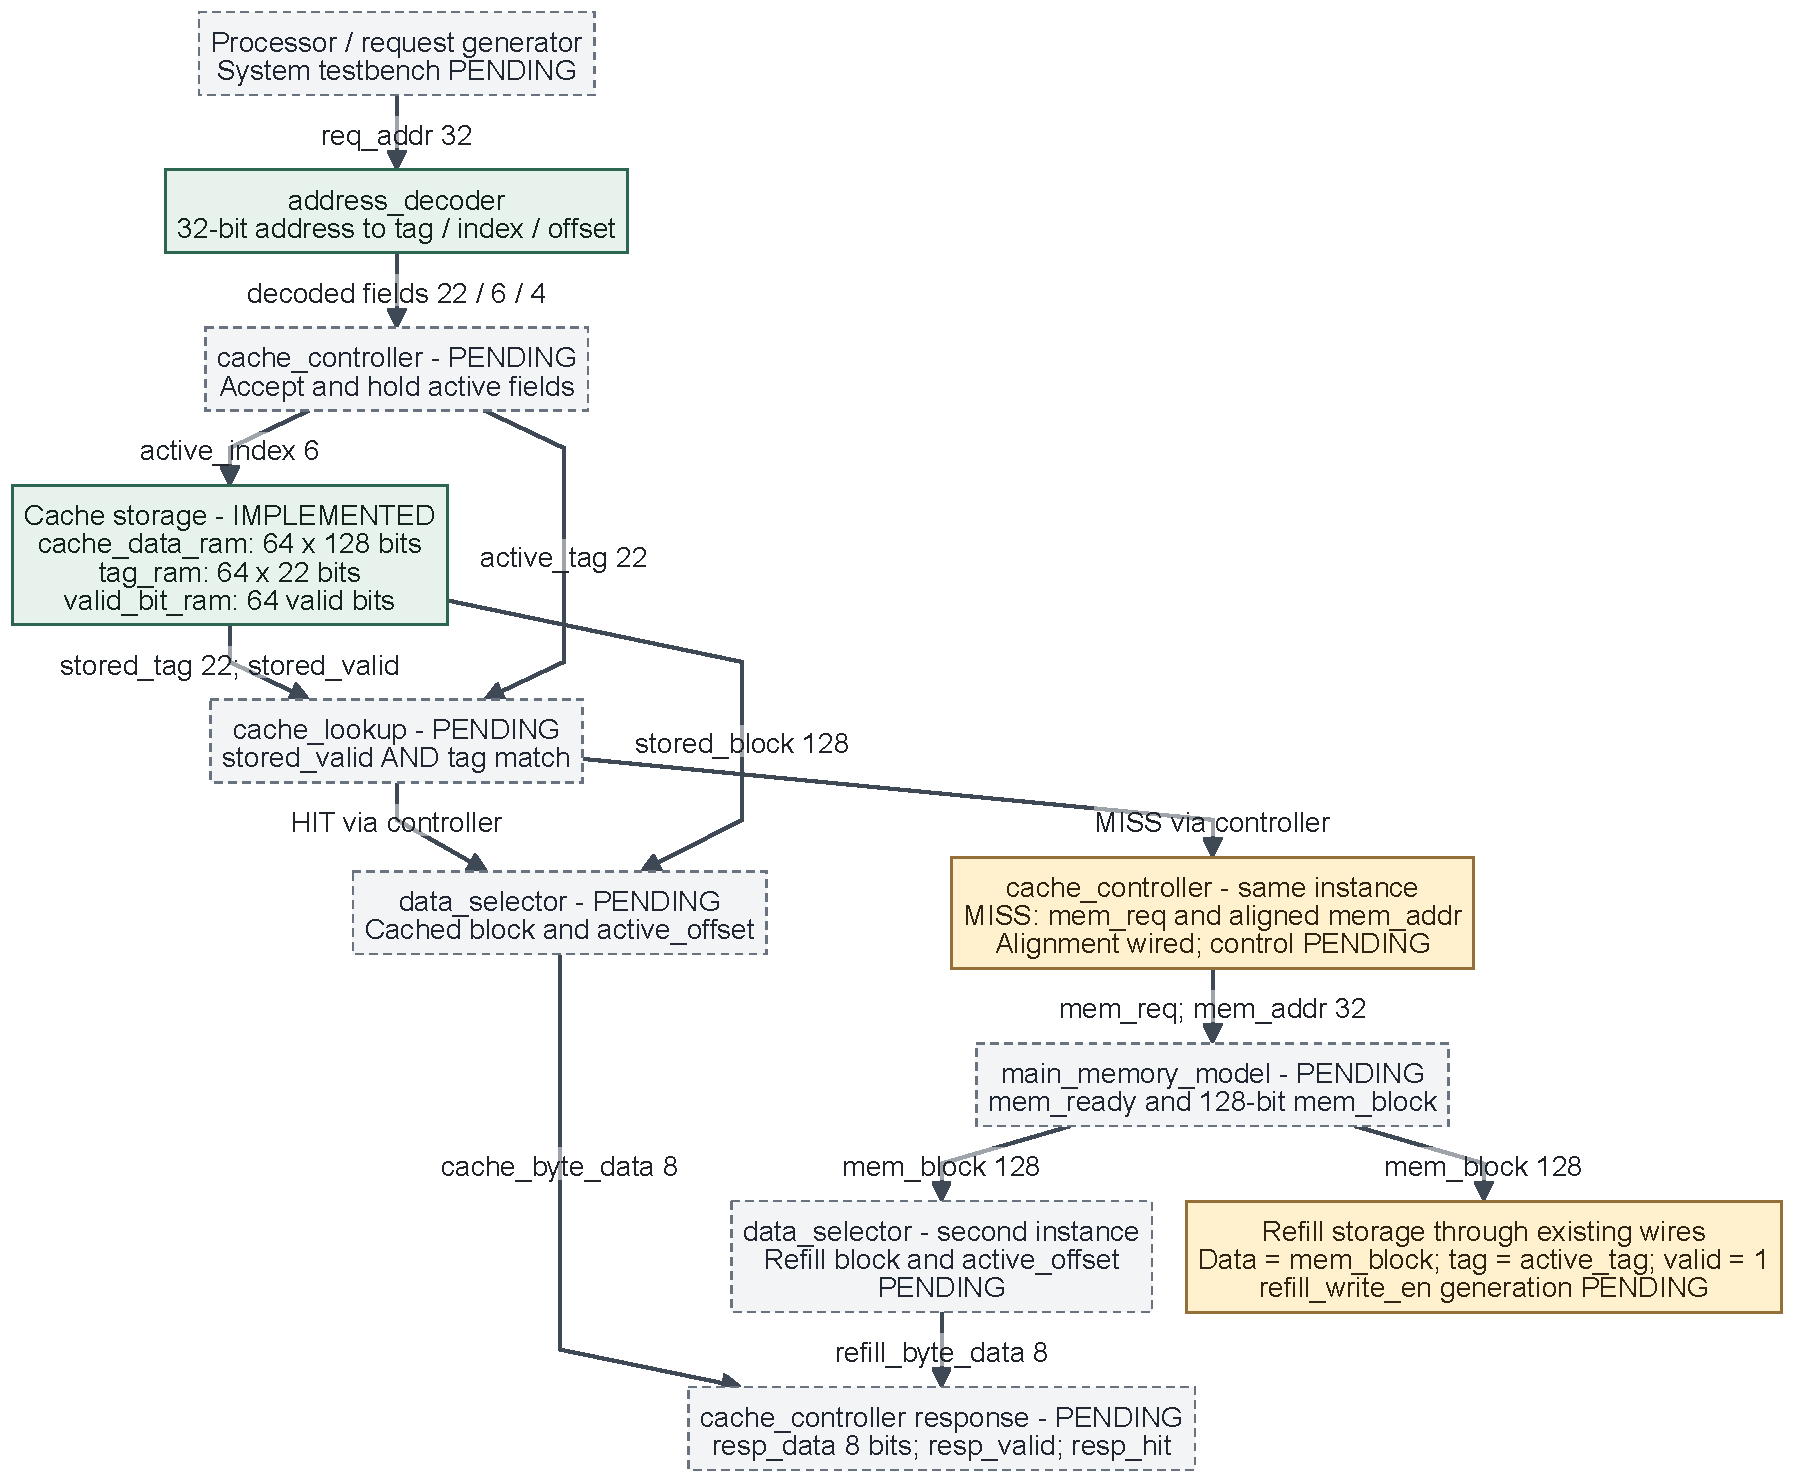
\includegraphics[width=0.98\textwidth,height=0.54\textheight,keepaspectratio]{system_architecture.pdf}
\caption{System architecture based on cache\_top boundaries. Green denotes implemented and independently tested primitives; amber denotes existing wiring with pending control; dashed gray denotes pending behavior. Repeated controller/storage views describe the same boundaries, not extra RTL instances.}\label{fig:system_architecture}
\end{figure}
\begin{figure}[!ht]
\centering
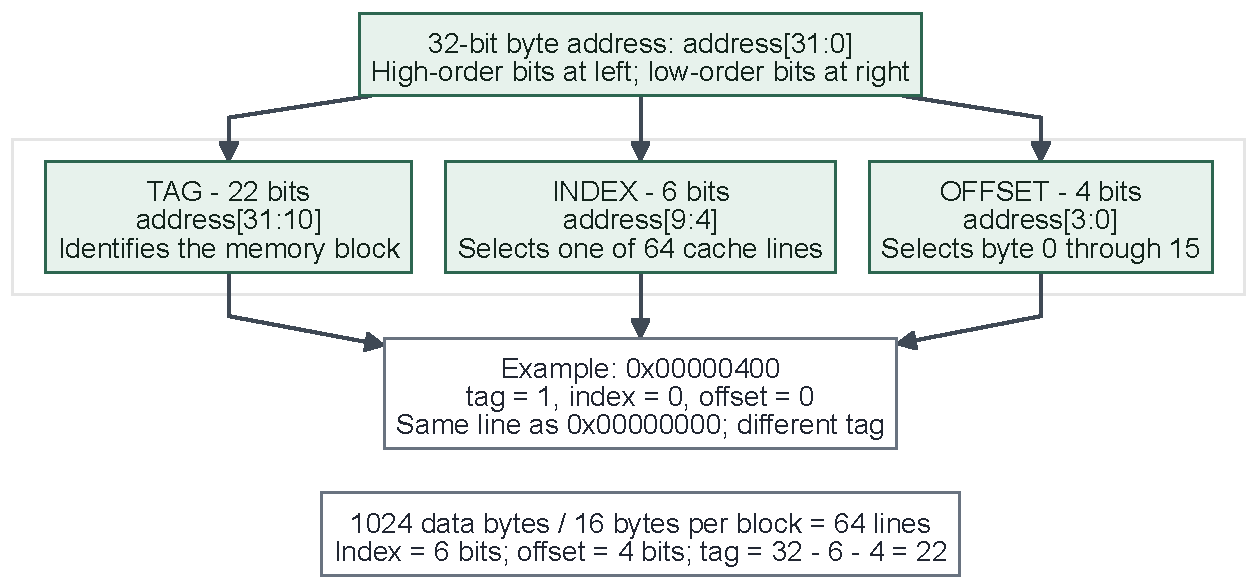
\includegraphics[width=0.98\textwidth,height=0.22\textheight,keepaspectratio]{address_breakdown.pdf}
\caption{Implemented 32-bit address split from address\_decoder.v. The tag distinguishes blocks sharing an index; the index selects a line; the offset identifies a byte. The worked example is a decoded address, not an observed cache miss.}\label{fig:address_breakdown}
\end{figure}
\clearpage
\begin{figure}[!ht]
\centering
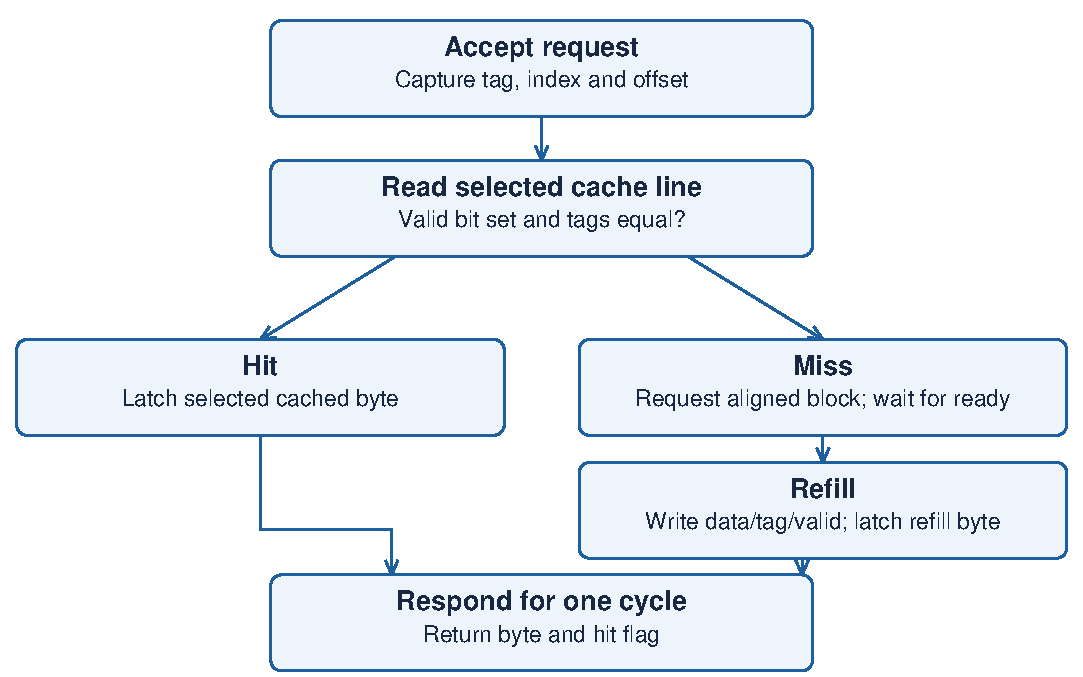
\includegraphics[width=0.98\textwidth,height=0.84\textheight,keepaspectratio]{cache_hit_miss_flow.pdf}
\caption{Proposed cache transaction flow from the interface contract. Address decoding and storage primitives exist. Acceptance, comparisons, hit/miss handling, memory service, refill sequencing and completion remain pending. Dashed decision nodes are not implemented logic.}\label{fig:cache_hit_miss_flow}
\end{figure}
\clearpage
\begin{figure}[!ht]
\centering
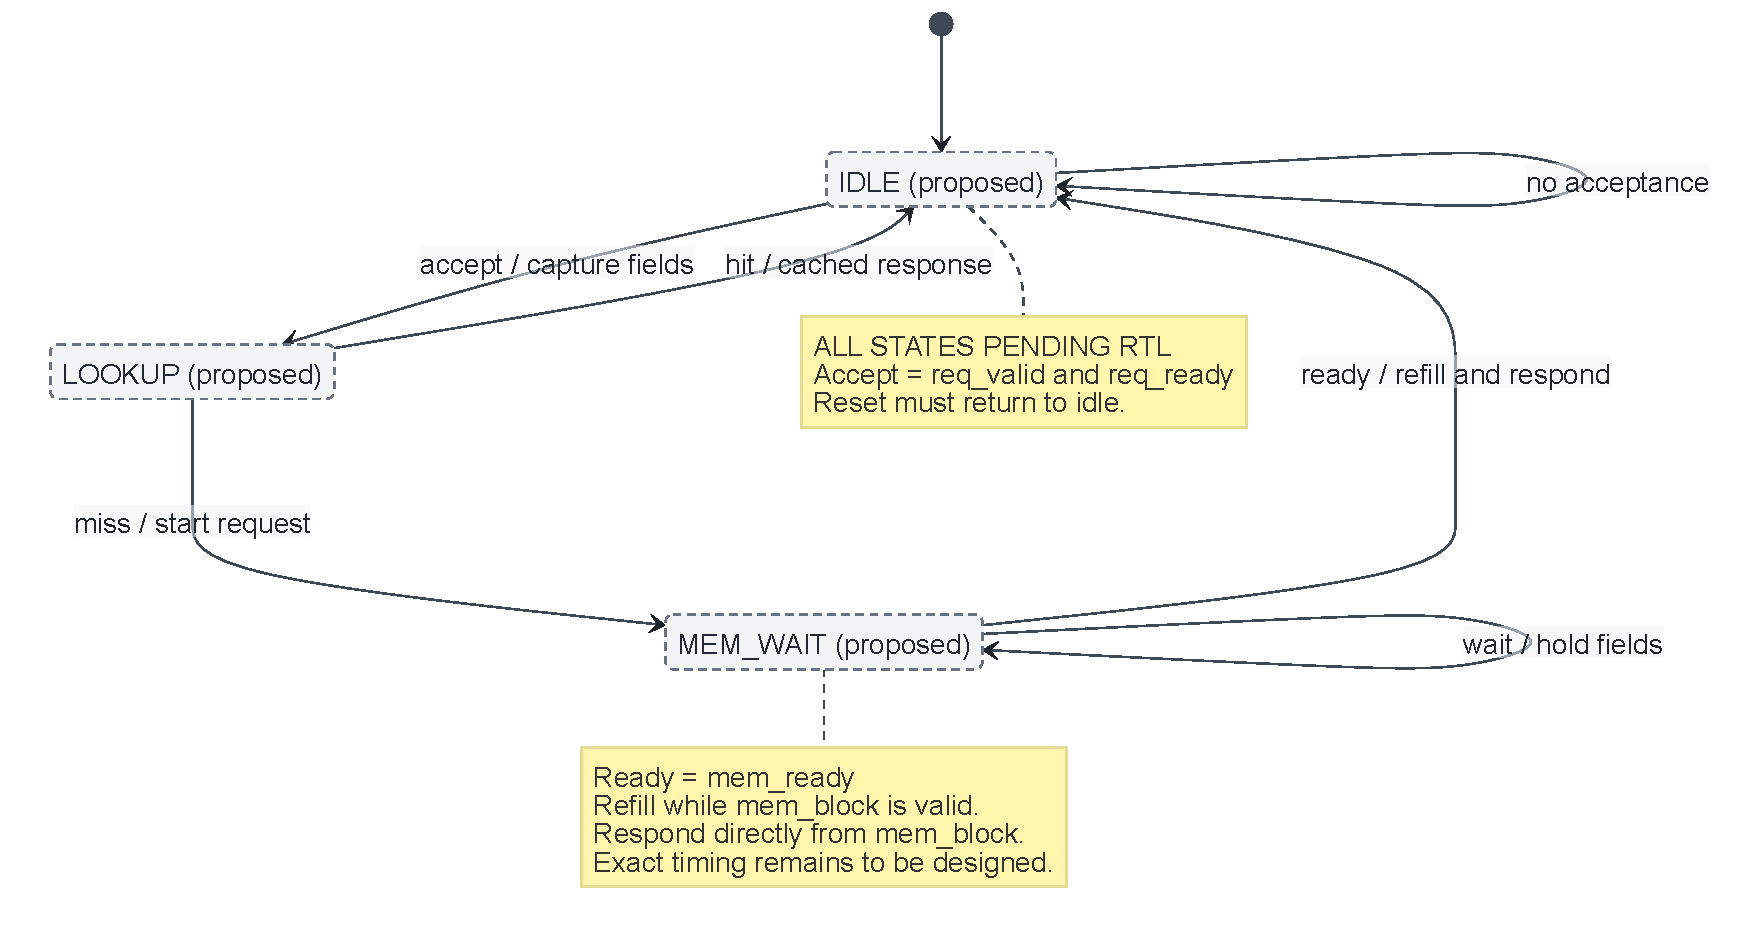
\includegraphics[width=0.98\textwidth,height=0.62\textheight,keepaspectratio]{controller_fsm.pdf}
\caption{Proposed controller state model, not extracted RTL. All states and transitions await implementation. The illustrative names originate in controller\_requirements.md; the refill/response transition must consume a valid returned block and preserve one response per request.}\label{fig:controller_fsm}
\end{figure}
\clearpage
\begin{figure}[!ht]
\centering
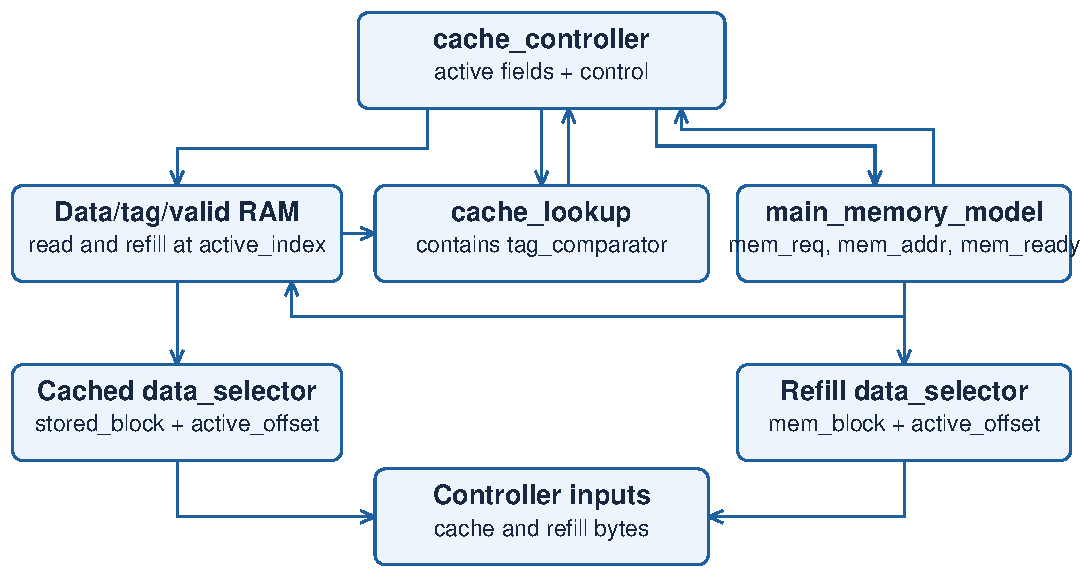
\includegraphics[width=0.98\textwidth,height=0.84\textheight,keepaspectratio]{module_connections.pdf}
\caption{Actual module instantiations and signal relationships in cache\_top.v. Views A and B repeat the same controller for readability. Dashed boxes are missing functional dependencies. The comparator is planned inside lookup and has no existing instance; common clock/reset connections are listed in the diagram.}\label{fig:module_connections}
\end{figure}
\clearpage
\end{document}
